\documentclass[tikz, border=10pt]{standalone}
\usetikzlibrary{positioning, arrows.meta}

\begin{document}
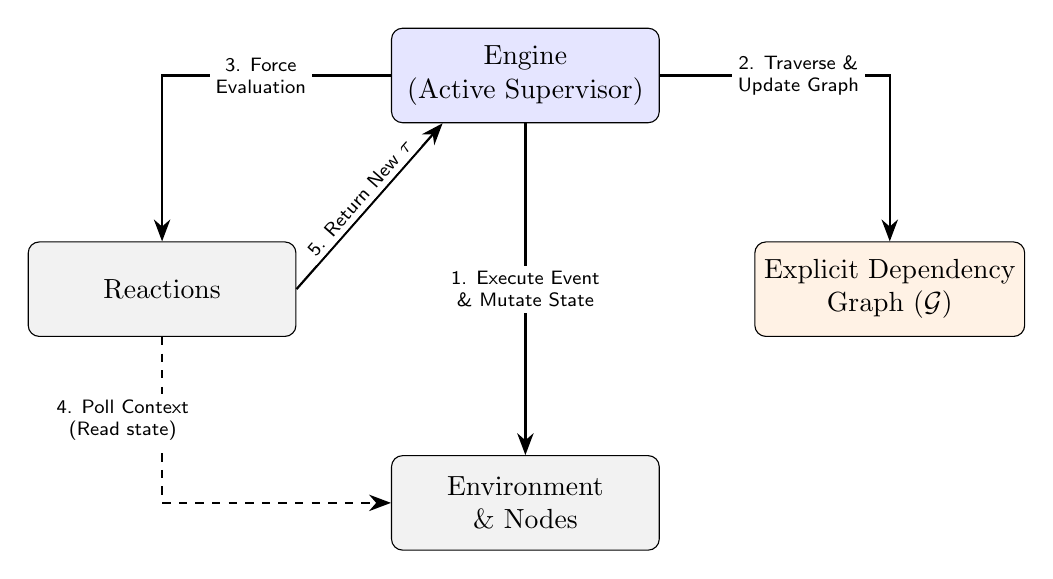
\begin{tikzpicture}[
    box/.style={draw, rectangle, rounded corners, minimum width=3.4cm, minimum height=1.2cm, align=center, fill=gray!10},
    arrow/.style={-{Stealth[scale=1.2]}, thick},
    dashed_arrow/.style={-{Stealth[scale=1.2]}, thick, dashed},
    lbl/.style={font=\sffamily\scriptsize, align=center, fill=white, inner sep=2pt}
]

% Nodes in a diamond layout
\node[box, fill=blue!10] (engine) {Engine \\ (Active Supervisor)};
\node[box, below right=1.5cm and 1.2cm of engine, fill=orange!10] (graph) {Explicit Dependency \\ Graph ($\mathcal{G}$)};
\node[box, below left=1.5cm and 1.2cm of engine] (react) {Reactions};
\node[box, below right=1.5cm and 1.2cm of react] (env) {Environment \\ \& Nodes};

% Centralized flow from the Engine
\draw[arrow] (engine.south) -- node[lbl] {1. Execute Event \\ \& Mutate State} (env.north);
\draw[arrow] (engine.east) -| node[lbl, near start, xshift=0.3cm] {2. Traverse \& \\ Update Graph} (graph.north);
\draw[arrow] (engine.west) -| node[lbl, near start, xshift=-0.2cm] {3. Force \\ Evaluation} (react.north);

% Reaction polling and returning
\draw[dashed_arrow] (react.south) |- node[lbl, near start, xshift=-0.5cm] {4. Poll Context \\ (Read state)} (env.west);
\draw[arrow] (react.east) -- node[lbl, sloped, above] {5. Return New $\tau$} (engine.210);

\end{tikzpicture}
\end{document}
